\documentclass{article}
\usepackage{graphicx}
\usepackage[normalem]{ulem}
\usepackage[margin=1.5cm]{geometry}
\usepackage{amsmath}

\begin{document}

\title{Laboratory on Restoring Forces}
\author{Prof. Jordan C. Hanson}

\maketitle

\begin{figure}[ht]
\centering
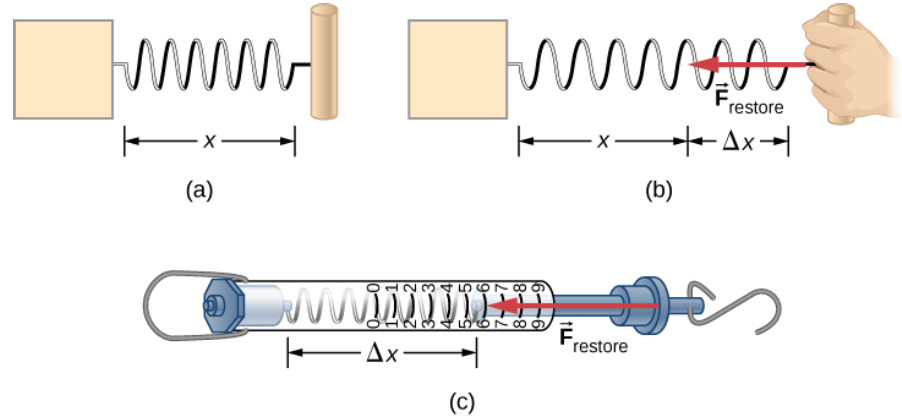
\includegraphics[width=0.35\textwidth]{figures/force1.png}
\caption{\label{fig:restore} An example of a restoring force generated by a spring.}
\end{figure}

\section{Restoring Forces, and Lab Setup}

The reason systems \textit{oscillate}, or move in a periodic fashion, is restoring force.  Consider Fig. \ref{fig:restore}.  When a spring is stretched by a displacement $\Delta \vec{x}$, the force applied is to the right and the force exerted by the spring is to the left.  The force exerted by the spring is called $\vec{F}_{\rm restore}$.  In today's laboratory, the relationship between $\Delta \vec{x}$ and $\vec{F}_{\rm restore}$ will be established.

At each station, there is a post with a hanging spring, a hook, a set of weights, and a meter stick.  Using the hook, weights may be hung from the spring such that it stretches.  Try hanging different weights on the spring to demonstrate that $\vec{F}_{\rm restore}$ is proportional to $\Delta \vec{x}$.

\section{Displacement of the Spring}

\begin{enumerate}
\item Measure the length of the \textit{spring} with the hook attached, and call this length $l_{0}$.  \underline{$l_{\rm 0}=$ \hspace{1cm} (cm)}
\item When the spring stretches, the length is increased.  The \textit{change in the length}, compared to $l_{\rm 0}$ is $\Delta \vec{x}$ (and the direction of the vector is down).  For example, if the spring is stretched downward to a new length of $10$ cm, and $l_{\rm 0} = 4$ cm, then $\Delta \vec{x} = -6$ cm.
\item Add successively larger masses to the hook, and record $\Delta \vec{x}$ in cm in Table \ref{tab:data}.
\begin{table}[hb]
\centering
\begin{tabular}{| c | c |}
\hline
Mass (grams) & $\Delta \vec{x}$ (cm) \\ \hline
 &  \\ \hline
 &  \\ \hline
 &  \\ \hline
 &  \\ \hline
 &  \\ \hline
 &  \\ \hline
 &  \\ \hline
 &  \\ \hline
 &  \\ \hline
 &  \\ \hline
 &  \\ \hline
\end{tabular}
\caption{\label{tab:data} Record data on the spring displacement versus mass here.}
\end{table}
\end{enumerate}

\section{Graphical Analysis}

\begin{enumerate}
\item The weight force due to gravity is $\vec{F}_g = -mg \hat{j}$, where $m$ is the mass (in kg) and $g = 9.81$ m s$^{-2}$.  Import the data in Tab. \ref{tab:data} into a spreadsheet, and compute the weight force created by the masses.
\item When the spring force balances the weight force, the mass is not moving and we conclude that the net force is zero.  That means the spring force magnitude equals the weight force magnitude, and it is in the opposite direction.  Plot the weight force versus $\Delta \vec{x}$ in the spreadsheet, and fit a trend line to the data.
\item What is the slope of the trend line? \underline{slope $=$ \hspace{1cm} (N/cm)} Is the trend line a good fit to the data?
\end{enumerate}

\section{Summary}

Based on the data collected, and the graphical analysis, write an equation that describes the restoring force of the spring:

\begin{equation}
\vec{F}_{\rm restore} = 
\end{equation}

\end{document}
